\subsubsection{Função Inversa da Tangente}

\begin{example}
Como $tan: \paren{- \frac {\pi} 2, \frac {\pi} 2} \to \R$ é
bijetiva, então essa função possui inversa, que chamamos de
\emph{arco tangente} e denotamos por $\arctan : \R \to
\paren{- \frac {\pi} 2, \frac {\pi} 2}$. Seu gráfico é mostrado na Imagem~\ref{img:grafico-arctan}.
%
\begin{figure}[H]
\centering
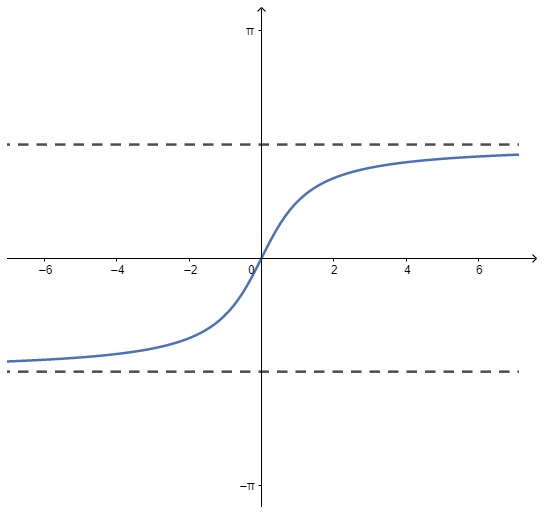
\includegraphics[scale=0.5]{\imgdirfromsection/grafarctan.jpg}
\caption{Gráfico da função $\arctan$.}
\label{img:grafico-arctan}
\end{figure}
\end{example}

\begin{onlineact}
	\khan{https://pt.khanacademy.org/math/trigonometry/trigonometry-right-triangles/reciprocal-trig-ratios/e/reciprocal_trig_funcs}{Razões Trigonométricas Recíprocas}.
\end{onlineact}

\begin{onlineact}
	\khan{https://pt.khanacademy.org/math/trigonometry/trigonometry-right-triangles/modeling-with-right-triangles/e/applying-right-triangles}{Problemas com Triângulos Retângulos}.
\end{onlineact}